\documentclass{article}
\usepackage[utf8]{inputenc}
\usepackage{graphicx}
\usepackage{listings}
\usepackage{booktabs}

\title{Lab 3}
\author{Hannah Atmer and Xiaoyue Chen \\ Team 6}
\date{October 2021}

\begin{document}

\maketitle

\section{Performance Estimates}
\subsection{Your estimates of the peak CPU and GPU performance and how you came up with them. }

  \begin{table}[h]
    \centering
    \begin{tabular}{p{0.3\textwidth}p{0.3\textwidth}p{0.4\textwidth}}
      \toprule
      Operation & Predicted performance & Why \\
      \midrule
      8-bit unsigned add & 787 GOPS & \(6 \times 4.1\times10^{9} \times 32 \times 1\) \\
      floating point add & 196 GFLOPS & \(6 \times 4.1\times10^{9} \times 8 \times 1\) \\
      Sequentially load a 32-bit int from an array & 3.6 GOPS & \(14.4 / 4\) \\
      Randomly load a 32 bit int from an array & 0.2 GOPS & \(14.4 / 16 / 4\) \\
      \bottomrule
    \end{tabular}
    \caption{Performance estimation for CPU}
  \end{table}

  \begin{table}[h]
    \centering
    \begin{tabular}{p{0.3\textwidth}p{0.3\textwidth}p{0.4\textwidth}}
      \toprule
      Operation & Predicted performance & Why \\
      \midrule
      8-bit unsigned add & 1734 GOPS & \(1280 \times 1.7 \times 1\) \\
      floating point add & 1734 GFLOPS & \(1280 \times 1.7 \times 1\) \\
      Sequentially load a 32-bit int from an array & 48 GOPS & \(192 / 4\) \\
      Randomly load a 32 bit int from an array & 1.5 GOPS & \(192 / 32
                                                            / 4\) \\
      Data transfer from CPU to GPU & 1.5 GB/s & measured \\
      \bottomrule
    \end{tabular}
    \caption{Performance estimation for GPU}
  \end{table}





% Answers about add benchmark
\subsection{Why were all benchmark runs not the same speed in 1 and 2?}

\subsection{What was the problem with 1 and 2 that we fixed in 3?}

\subsection{What optimization did the compiler do for 1 that prevented us from measuring what we wanted?}

\subsection{What did the code change in 2 do to prevent the compiler from doing this optimization?}

\subsection{What optimization did the compiler do for 3 that prevented us from measuring what we wanted?}

\subsection{Why was the performance of 4 so much slower than 2?}

\subsection{What was the optimization in 6 and why does it improve performance?}


% Results 
\section{Performance Achieved}

\subsection{Your measured performance results}

  \begin{table}[h]
    \centering
    \begin{tabular}{p{0.2\textwidth}p{0.2\textwidth}p{0.2\textwidth}p{0.2\textwidth}p{0.2\textwidth}}
      \toprule
      Operation & Predicted Max CPU Performance & Predicted Max CPU Performance & Max Measured CPU Performance & Max Measured GPU Performance \\
      \midrule
      8-bit unsigned add & 787 GOPS & 1734 GOPS & 354 GOPS & 41 GOPS \\
      floating point add & 196 GFLOPS & 1734 GFLOPS & 89 GFLOPS & 68 GFLOPS \\
      Sequentially load a 32-bit int from an array & 3.6 GOPS & 48 GOPS & .5 GOPS & 369 GOPS \\
      Randomly load a 32 bit int from an array & .2 GOPS & 1.5 GOPS & .009 GOPS & 1.3 GOPS \\
      Data transfer from CPU to GPU & & 1.5 GB/s & & 4.4 GB/s \\
      \bottomrule
    \end{tabular}
    \caption{Performance estimation for CPU}
  \end{table}

\subsection{Graph of results}

\begin{figure}[h!t]
    \centering
    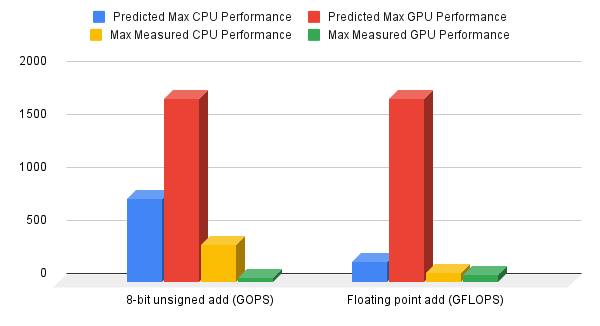
\includegraphics[width=1\textwidth]{add.png}
    \caption{Actual Performance Impact: Adding}
    \label{fig:add}
\end{figure}

\begin{figure}[h!t]
    \centering
    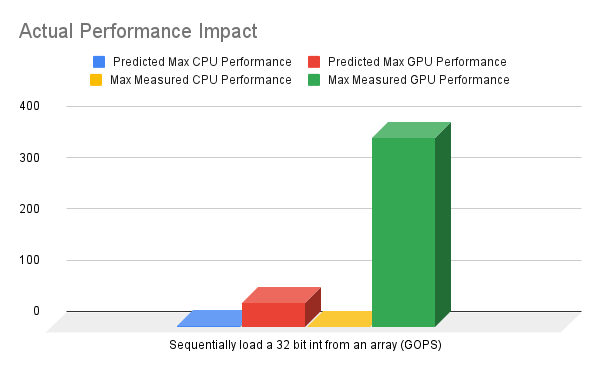
\includegraphics[width=1\textwidth]{sequential.png}
    \caption{Actual Performance Impact: Sequential Load}
    \label{fig:sequential}
\end{figure}

\begin{figure}[h!t]
    \centering
    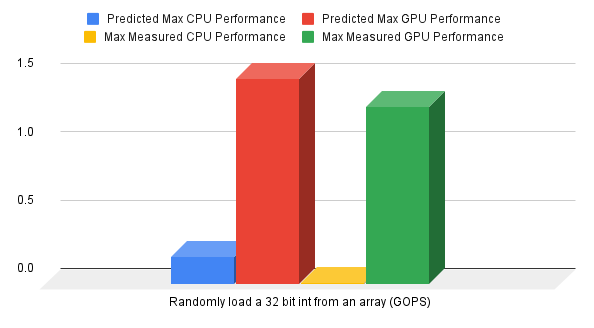
\includegraphics[width=1\textwidth]{random.png}
    \caption{Actual Performance Impact: Random Load}
    \label{fig:random}
\end{figure}

\begin{figure}[h!t]
    \centering
    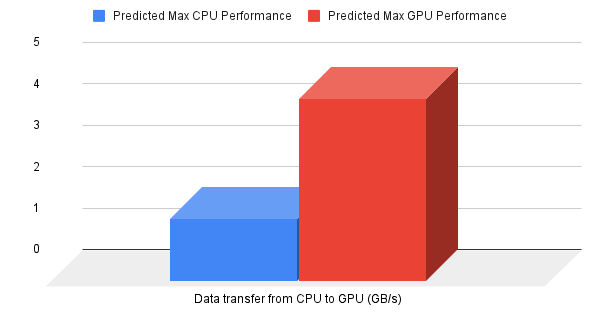
\includegraphics[width=1\textwidth]{dataTransfer.png}
    \caption{Actual Performance Impact: Data Transfer}
    \label{fig:transfer}
\end{figure}

% Discussion
\section{Discussion}

\subsection{A discussion of the measured results and how they differ
  from your predictions.}


\subsection{A discussion of what you learned about the hardware from measuring its performance.}

\subsection{A discussion of how you wrote your benchmarks and any issues you encountered and how you solved them.}



\subsection{Discuss how confident you are that your microbenchmarks accurately reflect the best obtainable performance.}

\subsection{Comment on any unexpected or odd results.}

\subsection{Comments on how this compares to your results from Labs 1 and 2 for the color conversion.}


\section{Lab comments}


\end{document}

%%% Local Variables:
%%% mode: latex
%%% TeX-master: t
%%% End:
